\chapter{Implementaciones experimentales}
\label{cap:implementacion}

A lo largo de este capítulo se mostrarán algunas de las aplicaciones desarrolladas para la obtención de las curvas de modulación del SLM, la presentación de máscaras al SLM y la simulación de los OVs, elementos que de alguna manera han facilitado, o bien el trabajo experimental o, la implementación de PD coherente.\\

% y finalmente, el montaje experimental, centrándonos en la caracterización del SLM.\\

En la sección \ref{sec:slm_carac} se analizará uno de los métodos de caracterización de modulación en fase y amplitud para un SLM de transmisión y su ejecución en el laboratorio, además se especificarán las características del LC-2002 y por último, se presentará una interfaz que se desarrolló para generar y proyectar máscaras en el SLM. Finalmente en la sección \ref{sec:mont_exp} se mostrará y analizará el montaje experimental.

% Caracterizacion SLM -
% Generacion de OVs simulados -
%	-> Empleando curva SLM -
% Montaje experimental -
% PD Coherente -
%	-> PD1 -
%	-> PD2 -
% Presentació de mascaras al SLM -
% 

\section{Caracterización del modulador espacial de luz}
\label{sec:slm_carac}
%Dado que para nuestros objetivos se requiere de la curva de caracterización del SLM, en esta sección discutiremos cómo puede obtenerse esta. 
Anteriormente se mencionó que la modulación depende del estado de polarización de la luz, tanto a la entrada del SLM como a la salida de éste; es necesario entonces contar con un sistema generador-analizador de estados de polarización \cite{Campos2000, Iemmi2001, Malacara2007}. Esto se realiza por medio de una lámina retardadora de media longitud de onda (HWP: \textit{HWP: half-wave plate}), un polarizador y dos láminas retardadoras de un cuarto de longitud de onda (QWP:\textit{quarter-wave plate}) configurados como sea se muestra en la Fig. \ref{fig:genpol}.

\begin{figure}[!ht]
  \centering
    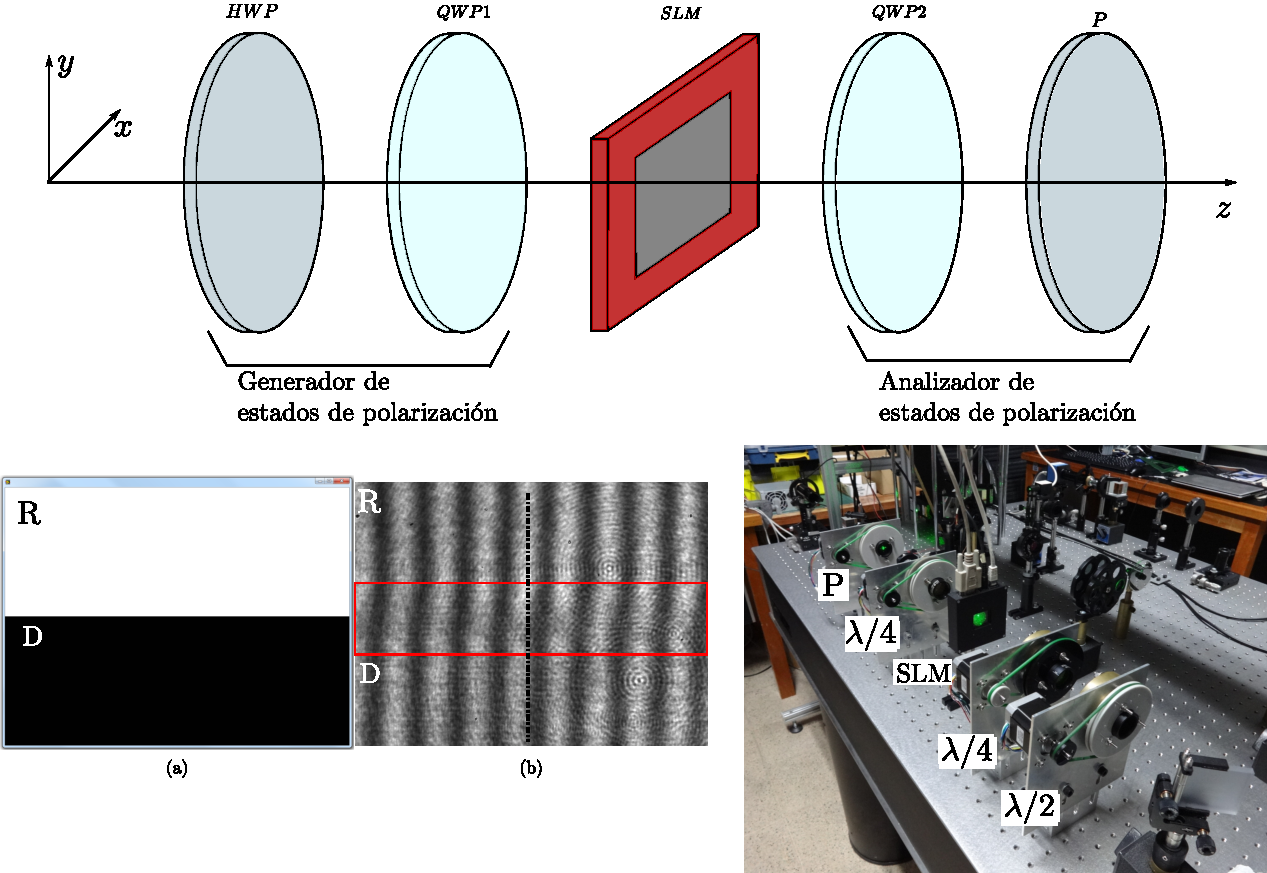
\includegraphics[width=\textwidth,keepaspectratio]{Caps/Imagenes/Gen-anPol.pdf}
  \caption{Estructura generador-analizador de estados de polarización para la caracterización de SLMs.}
  \label{fig:genpol}
\end{figure}

El generador de estados de polarización (PSG: \textit{polarization state generator}) se encarga de presentar el estado de polarización de la luz a la entrada del SLM, que puede ser lineal, circulares o elíptico, mientras que el analizador de estados de polarización (PSA: \textit{polarization state analyzer}) se encarga de analizar el estado de polarización a la salida del SLM. En conjunto, dadas las características de las moléculas de LC, según el estado de polarización puede haber una mayor o menor modulación de fase, amplitud o ambos. La caracterización del SLM se lleva a cabo a través de los resultados en intensidad medidos por un detector, en este caso, una cámara CCD, para diferentes estados de polarización, tanto en el analizador como en el generador de estados de polarización. La modulación en amplitud se determina a través del promedio de la intensidad medida \cite{Moreno2003, Ma2011}, mientras que la modulación en fase por su lado, se determina a través de un patrón de franjas interferométrico, en donde se divide el SLM en dos secciones, una de referencia y una en la cual se varía los niveles de gris en el SLM, el cambio en la fase produce entonces un desplazamiento del patrón de franjas en la sección donde se varían los niveles de gris con respecto a la sección referencia, como se muestra en la Fig.\ref{fig:faseslm}. \\

\begin{figure}[!ht]
  \centering
    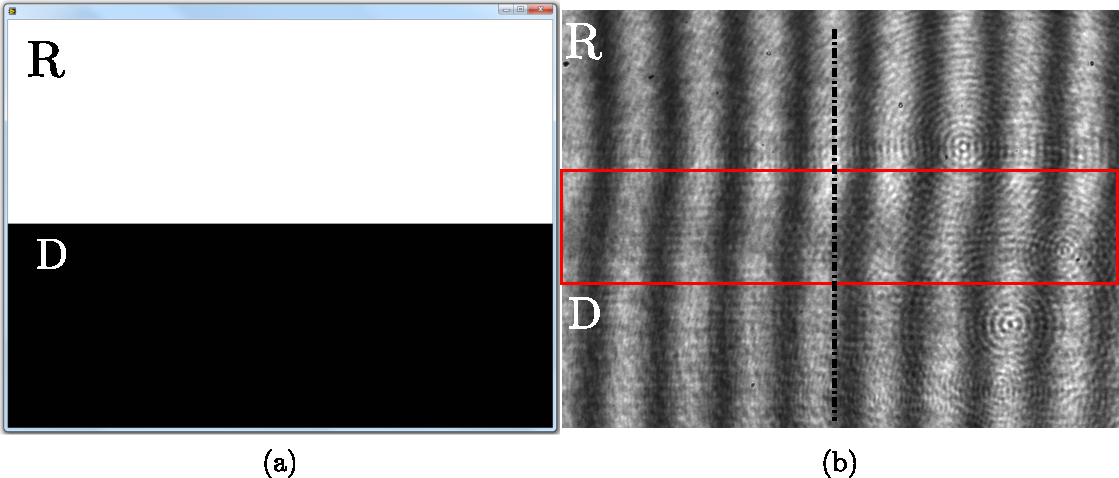
\includegraphics[width=14cm,keepaspectratio]{Caps/Imagenes/faseslm.pdf}
  \caption[Patrón de franjas para la determinación del corrimiento de fase en un sistema interferométrico.]{Patrón de franjas para la determinación del corrimiento de fase en un sistema interferométrico. (a) máscara dividida presentada al SLM, la sección R es la referencia y la sección D es en la que se varían los niveles de gris, y (b) patrón de franjas en el cual se desplaza la sección D a causa del cambio de fase producid por el SLM.}
  \label{fig:faseslm}
\end{figure}

Para llevar a cabo la caracterización, se diseñó un sistema compuesto por cuatro rotadores en donde cada uno de ellos se encarga de posicionar uno de los elementos ópticos; esto permite que la obtención de resultados experimentales sea de manera automática a través de una interfaz gráfica, en la cual solo es necesario ingresar qué estados se desean medir. Este sistema se muestra en la Fig. \ref{fig:rotadores}. Información detallada del proceso del modelo matemático que se sigue, resultados de la caracterización, hardware y software desarrollados puede encontrarse en la tesis de maestría de Santiago Echeverri \cite{EcheverriChacon2015}.

\begin{figure}[!ht]
  \centering
    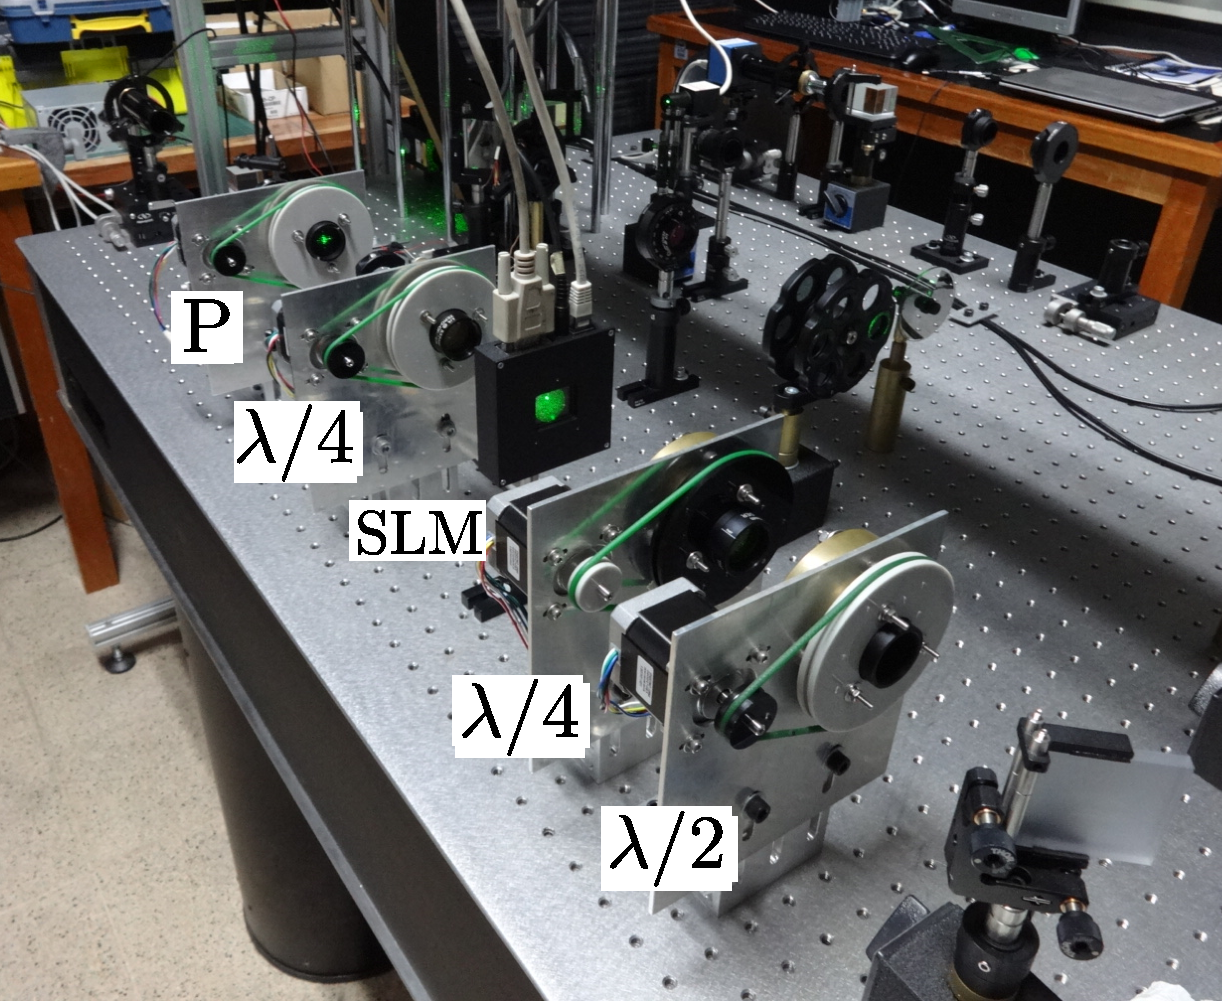
\includegraphics[width=12cm,keepaspectratio]{Caps/Imagenes/rotadores.pdf}
  \caption{Sistema de rotadores para la caracterización del SLM.}
  \label{fig:rotadores}
\end{figure}

El SLM que se emplea en este trabajo es un Holoeye LC-2002 (véase Fig. \ref{fig:lc2002}), el cual está basado en un microdisplay traslucido de LC y puede ser controlado electrónicamente vía computador\footnote{\url{http://www.rayscience.com/holoeye/LC2002_280.pdf}. }. En la Tabla \ref{tab:lc2002} se muestran las características técnicas.

\begin{figure}[!ht]
  \centering
    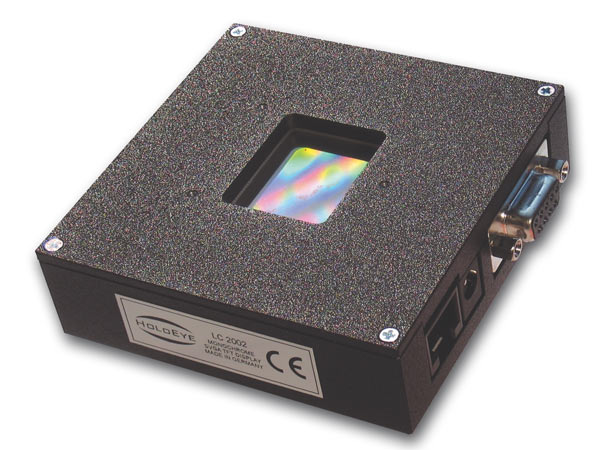
\includegraphics[scale=0.3]{Caps/Imagenes/lc2002.jpg}
  \caption[SLM HOLOEYE LC-2002.]{SLM Holoeye LC-2002. Imagen tomada de \small \url{http://holoeye.com/wp-content/uploads/2011/07/lc2002_spatial_light_modulator.jpg}}
  \label{fig:lc2002}		
\end{figure}



\begin{center}
\begin{table}
\centering
\begin{tabular}{|c|c|}
\hline 
Tipo de display & LC de transmisión \\ 
\hline 
Resolución & 800$\times$600 \\ 
\hline 
Tamaño del píxel & 32 $\mu$m \\ 
\hline 
Factor de llenado & $55\%$ \\ 
\hline 
Área activa & 21$\times$26mm \\ 
\hline 
Modulación de fase & $2\pi$ a 532nm \\ 
\hline 
\end{tabular} 
\caption{Características del LC-2002}
\label{tab:lc2002}
\end{table}
\end{center}

Para facilitar la generación y presentación de máscaras al SLM, se incorporaron las diferentes funciones que generan máscaras en una sola aplicación denominada ``SLM Mask Generator'', como se muestra en la Fig. \ref{fig:maskgen}. Esta se ha desarrollado en Matlab y se encuentra en proceso de registro de software ante la Dirección Nacional de Derecho de Autor.\\

\begin{figure}[!ht]
  \centering
	    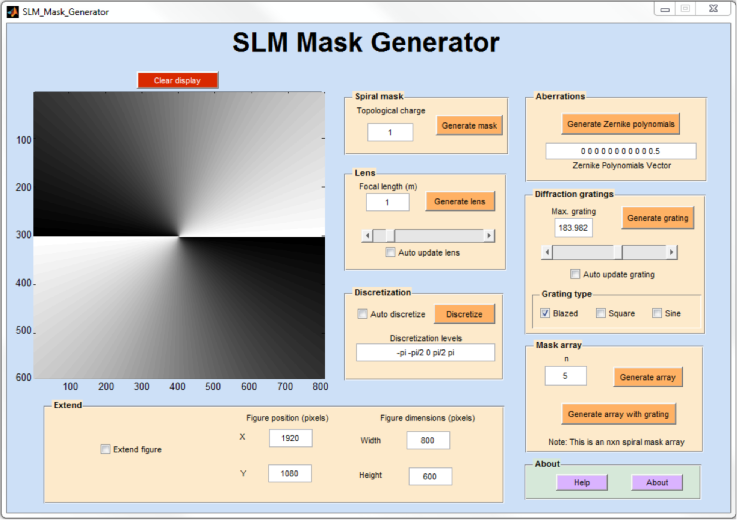
\includegraphics[width=\textwidth,keepaspectratio]{Caps/Imagenes/maskgen.png}
	\caption[Interfaz para la generación de máscaras.]{Interfaz para la generación de máscaras con diversas características para presentarse al SLM.}
	\label{fig:maskgen}
\end{figure}

La generación de una máscara espiral de fase se realiza mediante el ingreso de una carga topológica en la casilla ``Topological charge'' y posteriormente, haciendo click en el botón ``Generate mask'', con esto se dará una vista previa de la máscara como la que se muestra en el recuadro. A través de la opción ``Extend'' puede presentarse la máscara al SLM, esto debido a que cuando el SLM está conectado al computador funciona como una segunda pantalla y puede entonces cambiar el tamaño y la posición de la imagen a proyectar. A grandes rasgos, la aplicación permite simular diferentes tipos de elementos de fase como: aberraciones a partir de los polinomios de Zernike, redes de difracción de tres tipos e incluso, arreglos de máscaras espirales. En la Fig. \ref{fig:resmaskapp} se presenta el resultado para cuatro máscaras generadas con la aplicación.

%Para presentar las diferentes máscaras al SLM implementó una interfaz gráfica en MATLAB, que se muestra en la Fig.\ref{fig:maskgen}, la cual permite generar máscaras con diversas características, entre las cuales se tiene:

%\begin{itemize}
%	\item Genera máscaras espirales de cualquier carga topológica que son ajustables a la resolución del modulador espacial.
%	\item Extender las máscaras con una sección de posicionamiento y ajuste del tamaño, en donde se puede decidir la posición y dimensiones de la máscara a proyectar
%Permite superponer lentes de diferentes distancias focales a la máscara actual y posee una opción de actualización automática en caso de que se desee variar la distancia focal de manera dinámica. 
%	\item Puede discretizar las máscaras en niveles de gris, estos niveles permiten la creación de máscaras de dos o más niveles de gris, esta sección también la posibilidad de discretizar de manera automática. 
%	\item Genera aberraciones a partir de los polinomios de Zernike, en donde dado un vector de pesos se genera una superficie con la suma de las características de los pesos y se superpone a la máscara actual. 
%Produce redes de difracción de tres tipos: binarias, sinusoidales o diente de sierra, en las cuales se puede variar el periodo de manera dinámica.
%	\item Posee una sección para la generación de arreglos de nxn máscaras espirales y a estos arreglos puede añadirse redes de difracción.
%\end{itemize}



\begin{figure}[!ht]
  \centering
	    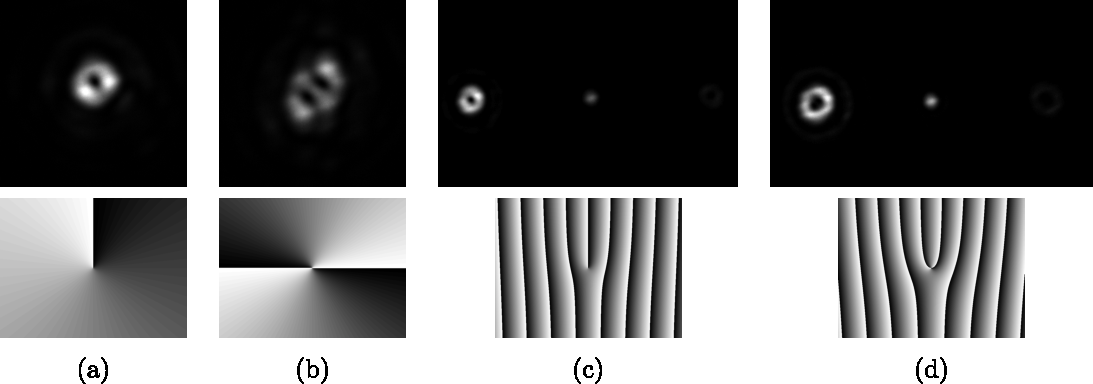
\includegraphics[width=\textwidth,keepaspectratio]{Caps/Imagenes/resmaskapp.pdf}
	\caption[Resultados de máscaras generadas con el ``SLM Mask Generator''.]{Resultados de máscaras generadas con el ``SLM Mask Generator''. (a) Máscara de fase espiral con carga topológica $l=1$, (b) máscara de fase espiral $l=2$, (c) red de difracción diente de sierra bifurcada con $l=1$ y (d) red de difracción diente de sierra bifurcada con $l=2$.}
	\label{fig:resmaskapp}
\end{figure}

%\section{Presentación de hologramas generados por computadora al modulador espacial de luz}

%Como el SLM también posee las características de un LCD, la presentación de las diferentes máscaras puede realizarse a través de una interfaz

%\section{Simulación de vórtices ópticos}
%\label{sec:gen_vor_sim}
%
%Ahora bien, puesto que PD coherente requiere de una estimación \textit{a priori} del objeto, lo que allí se hace es emplear un simulador de OVs, un diagrama de flujo de este se muestra en la Fig. \ref{fig:GenVor}a. El proceso que se sigue es en esencia el propuesto en la Eq.\ref{eqD1}, es decir, una convolución entre el plano objeto y la función de punto extendido. Puesto que en la propuesta de PD1 y PD2 se opta por modificar la simulación de forma tal que la fase que es añadida por la función pupila generalizada concuerde con los valores de modulación de fase real\footnote{Recordemos que las variaciones de intensidad se desprecian puesto que el estado de polarización es tal que las variaciones de intensidad son mínimas.} se añade un paso adicional a la simulación, en el cual los valores de fase son modificados para que estos correspondan a los valores de fase aportados por el SLM (Fig.\ref{fig:GenVor}b). Dado que queremos realizar una convolución, uno de los sistemas ópticos más empleado para ello ha sido el bien conocido correlador 4F.En este se siguen las siguientes etapas: se tiene un par de lentes cada una con distancia focal $f$, primero se ubica una de ellas a una distancia $f$ del plano objeto, de forma que a $2f$ de se genere la transformada de Fourier del plano objeto. En este punto se añade la PSF del sistema, que en nuestro caso corresponde a la información de fase añadida por el SLM. A continuación se ubica la segunda lente a una distancia de $3f$ con respecto al plano objeto, esta se encargará de realizar una segunda transformadad de Fourier del producto entre la PSF y la transformada del plano objeto, de forma que a la salida lo que tendremos de acuerdo a la Eq.\ref{eqD1} es la convolución entre la  PSF y el plano objeto.
%
%\begin{figure}[!ht]
%  \centering
%  	\subfigure[Sin modulación real.]{
%	    \includegraphics[scale=1]{Caps/Imagenes/GenVor.pdf}}
%	\quad
%	\subfigure[Con modulación real.]{
%	    \includegraphics[scale=1]{Caps/Imagenes/GenVorMod.pdf}}
%	\caption{Simulación de OVs.}
%	\label{fig:GenVor}
%\end{figure}


%\begin{figure}[!ht]
%  \centering
%    \includegraphics[scale=1]{Caps/Imagenes/GenVorMod.pdf}
%  \caption{Diagrama de flujo de la simulación de un OV modificado para emplear la}
%  \label{fig:montaje}
%\end{figure}

\section{Montaje experimental}
\label{sec:mont_exp}

%Un esquema del montaje se presenta en la Fig. \ref{fig:montaje}, el cual está compuesto por un interferómetro Mach-Zehnder que en uno de sus brazos ha sido ubicado un correlador 4F. Además, en el 4F se ha ubicado el sistema PSG-PSA de forma que con uno de los brazos del intereferométro se hace imagen de un punto objeto y  se añade el SLM que se encarga de presentar los CGH. La Fig.\ref{fig:montexp} es una toma del montaje físico.

%Un esquema del montaje se presenta en la Fig. \ref{fig:montaje}, como fuente de iluminación se emplea un láser de estado sólido con una longitud de onda de $532$nm, con polarización vertical y modo $TEM_{0,0}$. Primero se ubica un polarizador con recubrimiento delgado a base de nanopartículas con alta relación de extinción ($10000:1$) de referencia LPVISB050 fabricado por THORLABS; este polarizador se utiliza ya que los láseres de estado sólido pueden tener una polarización elíptica. A continuación se sitúa un filtro de densidad neutra que permite modificar la intensidad y a través de un conjunto de espejos de primera superficie, se lleva el haz hasta un filtro espacial compuesto por un objetivo de $10\times$ y un ``pinhole'' de $5\mu $m, que permite filtrar las altas frecuencias y producir un haz Gaussiano. Luego se ubica una lente colimadora con distancia focal de $10$cm, seguido por un divisor de haz no polarizado de referencia $49-004$ fabricado por Edmund Optics, desde aquí se genera entonces un interferómetro Mach-Zehnder. En el brazo objeto se ubica una primera lente tiene una distancia focal de $10$cm, de forma que en el plano focal de dicha lente tendremos el plano objeto, a partir de este se da entonces el sistema formado de imagen 4F. Se ubica una segunda lente de forma que a distancia focal está colocado el SLM, garantizando que las fases introducidas por el SLM están en un plano de Fourier. Antes de este está el sistema PSG conformado por una lámina de cuarto de longitud de onda de referencia WPQ10M-532 de THORLABS y una lámina de media longitud de onda de referencia WPH10M-532 del mismo fabricante. Después del SLM está el PSA conformado por un polarizador y una lámina de cuarto de onda. Se ubica una segunda lente de forma que desde el SLM hasta el plano imagen hay $2f$ y allí se ubica un ocular mar Newport con aumento de $10\times$ acoplado a una cámara CCD marca Imaging Source modelo DMK 41BU02.H con una resolución de $1280 \times 960$. 

Un esquema del montaje se presenta en la Fig. \ref{fig:montaje}, como fuente de iluminación se emplea un láser de estado sólido con una longitud de onda de $532$nm, con polarización vertical y modo $TEM_{0,0}$. Primero se ubica un polarizador con recubrimiento delgado a base de nanopartículas con alta relación de extinción ($10000:1$) de referencia LPVISB050 fabricado por THORLABS; este polarizador se utiliza ya que los láseres de estado sólido pueden tener una polarización elíptica. A continuación se sitúa un filtro de densidad neutra que permite modificar la intensidad y a través de un conjunto de espejos de primera superficie, se lleva el haz hasta un filtro espacial compuesto por un objetivo de $10\times$ y un ``pinhole'' de $5\mu $m, que permite filtrar las altas frecuencias y producir un haz Gaussiano. Luego se ubica una lente colimadora con distancia focal de $10$cm, seguido por un divisor de haz no polarizado de referencia $49-004$ fabricado por Edmund Optics. En el brazo objeto se ubica una primera lente, con una distancia focal de $10$cm, de forma que en el plano focal de dicha lente tendremos el plano objeto. Se ubica una segunda lente de forma que a distancia focal está situado el SLM, garantizando que las fases introducidas por el SLM están en un plano de Fourier. Antes de este está el generador de estados de polarización conformado por una lámina de cuarto de longitud de onda de referencia WPQ10M-532 de THORLABS y una lámina de media longitud de onda de referencia WPH10M-532 del mismo fabricante. Después del SLM está el analizador de estados de polarización conformado por un polarizador y una lámina de cuarto de onda. Se ubica una segunda lente de forma que desde el SLM hasta el plano imagen hay $2f$ y allí se ubica un objetivo de microscopio Newport con aumento de $20\times$ acoplado a una cámara CCD marca Imaging Source modelo DMK 41BU02.H con una resolución de $1280 \times 960$. 


\begin{figure}[!ht]
  \centering
    \includegraphics[width=\textwidth,keepaspectratio]{Caps/Imagenes/Montaje.pdf}
  \caption{Esquema del montaje experimental.}
  \label{fig:montaje}
\end{figure}



\begin{figure}[!ht]
  \centering
    \includegraphics[width=\textwidth,keepaspectratio]{Caps/Imagenes/montexp.JPG}
  \caption{Montaje experimental.}
  \label{fig:montexp}
\end{figure}

